\documentclass[12pt]{report}
\usepackage[utf8]{inputenc}
\usepackage[francais]{babel}
\usepackage[T1]{fontenc}
\usepackage{amsmath}
\usepackage{amsfonts}
\usepackage{amssymb}
\usepackage{graphicx}
\usepackage{titlesec}
\usepackage{caption}

\graphicspath{ {../img/} }
\titleformat{\chapter}[hang] {\normalfont\huge\bfseries}{\thechapter. }{}{}

\begin{document}
\begin{titlepage}

\title{
	{\Huge Cahier des charges}\\
	{\large Brainless Devs}\\
	{\vspace{2em}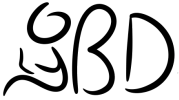
\includegraphics[center]{logo_short.png}}
}
\author{
	Thibault Allançon\\
	Valérian Fayt
	\and
	Antoine Gonzalez\\
	Cédric Parpet}
\date{
	\vfill 
	Dossier Projet Informatique\\
	Info-Sup EPITA\\
	Janvier 2018
}

\maketitle

\tableofcontents

\chapter{Introduction}

\begin{figure}
\centering
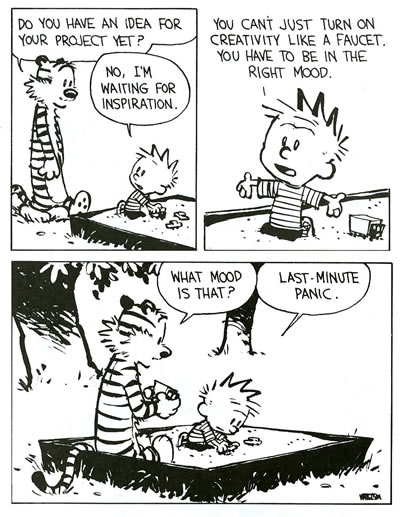
\includegraphics[width=0.6\textwidth]{project_mood}
\caption*{\textit{Calvin and Hobbes}, Bill Watterson}
\end{figure}

\chapter{Origine du projet}

\section{Présentation de l'équipe}
\section{Inspirations}

\chapter{Description du gameplay}

\section{Carte et ressources principales}

La carte sera découpée en tuiles hexagonales, et sera générée procéduralement.  Les cases seront organisées par groupements de même biome, ayant chacun des caractéristiques particulières. Le biome forêt réduira par exemple la portée de vue des unités ainsi que leurs déplacements, le biome océan empêchera toutes constructions, ou le biome montagne bloquant tous déplacements d'unités.\\

Comme dans la grande majorité des jeux de stratégies aujourd'hui, nous mettrons en place un brouillard de guerre afin de rajouter un côté exploration dans le jeu (chercher les ressources, chercher les ennemis). Construire un  bâtiment ou déplacer une unité dans le brouillard de guerre révèlera une partie de la carte (dans un rayon autour de l'unité correspondant à une portée de vue) tant qu'ils existeront.\\

La carte contiendra également des ressources que le joueur devra exploiter afin de progresser. Ces ressources sont divisées en deux catégories: ressources stratégiques et ressources de luxe. Les ressources stratégiques (métaux, chevaux...) serviront à construire et améliorer des bâtiments et unités tout au long de la partie. Les ressources de luxe (or, diamant...) seront indispensables pour garantir une stabilité économique, sans laquelle le joueur subira des révoltes, traduits en partie par des malus comme une réduction de production de richesses et une augmentation plus lente de la population. 

\section{Fonctionnement des unités}

Le colon est une unité importante pour la progression du joueur: il sert à fonder une nouvelle ville. Il s'agira d'une unité couteuse, et extrêmement vulnérable car sans défenses. Il devra être utilisé avec précaution.\\

Les ouvriers sont les unités sans défense qui construisent les exploitations de ressources sur les cases en contenant. Leur coût est relativement faible, et il est possible de capturer les ouvriers d'un adversaire.\\

Les militaires sont les seules unités capables de piller des cases de ressources, détruire des villes, et tuer ou capturer des unités. Il sera possible de les améliorer au cours de la partie.

\section{Caractéristiques des villes}

Les villes représentent un aspect important de la partie : elles constituent l'empire du joueur, et permettent notamment la création d'unités, de bâtiments, ainsi que la génération de richesses. \\

Les villes possèderont une population croissante, dont dépendra leur production: l'argent, la science, et la productivité. Cette population devra être satisfaite en ressources de luxe, sans quoi elle sera mécontente et moins performante.\\

Les richesses produites par les villes serviront à construire des bâtiments, créer des unités, et déverrouiller des améliorations. La science et l'argent seront unifiées entre les villes, mais la productivité sera propre à chaque ville.\\

La science fonctionnera comme un système d'expérience: le joueur en obtiens une certaine quantité chaque tour, et elle déverrouillera l'accès à certaines améliorations ou fonctionnalités en atteignant des paliers.

\section{Déroulement d'une partie}

Le joueur commence la partie avec un colon et un guerrier, et doit construire sa première ville. Il devra ensuite se développer tout au long de la partie, en construisant d'autres villes, cherchant des ressources sur la carte, et en créant une force militaire.\\

Le joueur sera amené à se battre contre les adversaires, qui en solo prendront la forme de tribus barbares contrôlées par une IA. La partie se termine lorsqu'un joueur effectue une victoire militaire (en multijoueur uniquement) qui implique de détruire toutes les villes des adversaires, ou une victoire scientifique qui consiste atteindre le dernier pallier de Science. Un joueur a perdu lorsque toutes ses villes sont détruites.

\chapter{Conception et aspects techniques}

\chapter{Répartition des tâches}

\chapter{Conclusion}

\chapter{Références}

\end{document}
